\newpage
\section{Aufbau}
\label{sec:Aufbau}
Der in diesem Versuch verwendete Aufbau ist in Abbildung \ref{abb:aufbau} dargestellt.
\begin{figure}[htb]
  \centering
  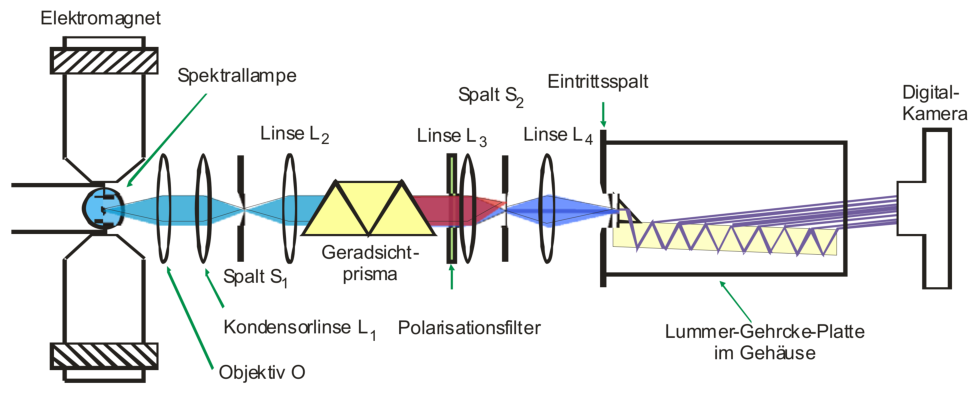
\includegraphics[width=0.8\textwidth]{images/V27_7.pdf}
  \caption{Graphische Darstellung des Aufbaus zur Untersuchung des Zeemann-Effektes \cite{anleitung}.}
  \label{abb:aufbau}
\end{figure}
Als Strahlungsquelle wird eine Cd-Lampe verwendet. Diese ist zwischen den Polen
eines Elektromagneten befestigt. Der Magnet sorgt dafür, dass die Emissionslinien
der Cd-Lampe aufgespalten werden. Weitere Linsen, sowie der Spalt(S1) verstärken
diesen Effekt. Ein
Geradsichtprisma sorgt für eine Separation der Wellenlängen voneinander. Dabei
werden die Wellenlängen in räumlich horizontaler Richtung voneinander getrennt,
sodass ein Verschieben von Linse L3 und des Spaltes S2 eine Auswahl der Wellenlängen
erlaubt, die auf den Eintrittsspalt der Lummer-Gehrcke-Platte fällt. Durch einen
eingesetzten Polarisationsfilter, können die $\sigma$-Linien separat von den
$\pi$-Linien untersucht werden. Dazu muss der Polarisationsfilter um \SI{90}{\degree}
gedreht werden.
\begin{figure}[htb]
  \centering
  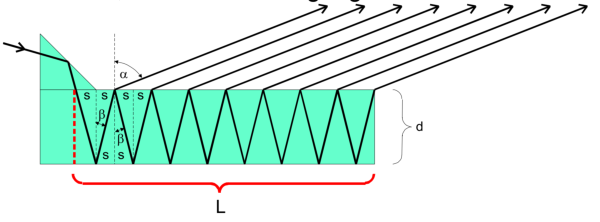
\includegraphics{images/V27_6.pdf}
  \caption{Graphische Darstellung der Lummer-Gehrcke-Platte \cite{anleitung}.}
  \label{abb:lummer}
\end{figure}
Eine Lummer-Gehrcke-Platte besteht aus mehreren planparallelen Platte, die bei
auftreffen von monochromatischer Strahlung ein Interferenzmuster erzeugt. Wie in
Abbildung \ref{abb:lummer} dargestellt wird der einfallende Lichtstrahl über ein
geeignetes Prisma in die Platte reflektiert. Durch Reflektion an der Außenschicht
des Glasses tritt ein kleiner Teil des Lichtes aus dem Glass aus und interferiert
mit Strahlenbündeln anderer Reflexionen. Für eine konstruktive Interferenz muss
die Bedingung
\begin{align*}
  2d\cdot \cos{\theta} = n\lambda
\end{align*}
erfüllt sein. $d$ entspricht dabei der Plattendicke und $\lambda$ der Wellenlänge
des einfallenden Strahls. Die hier verwendete monochromatischer Strahlung wird
formt Unterferenzstreifen. Zusätzlich sorgt das eingeschaltete Magnetfeld dafür,
dass die Wellenlängen um $\delta\lambda$ und die Interferenzstreifen um $\delta s$
verschiebt. Um eine Überlagerung von zwei Wellenlängen unterschiedlicher Ordnung
zu vermeiden, darf eine Wellenlängendifferenz
von
\begin{align*}
  \Delta\lambda_\text{D} = \frac{\lambda^2}{2d}\dot\frac{1}{\sqrt{n^2-1}}
\end{align*}
zwischen zwei Wellenlängen nicht überschritten werden. Das Auflösungsvermögen der
Lummer-Gehrcke-Platte wird beschrieben durch die Länge $L$ und dem Brechungsindex
$n$ mit
\begin{align*}
  A = \frac{\lambda}{\Delta\lambda} = \frac{L}{\lambda}\left(n^2-1\right).
\end{align*}
Die von der Lummer-Gehrcke-Platte ausgehenden Interferenzstreifen werden mit Hilfe
einer Digitalkamera aufgenommen.

\section{Durchführung}
\label{sec:Durchführung}
Bevor der Versuch durchgeführt werden kann, muss der Aufbau aus \ref{sec:Aufbau}
vorbereitet und die Optik justiert werden. Es ist darauf zu achten, dass sowohl
das Geradenprisma als auch die Lummer-Gehrcke-Platte nicht von ihrer Halterung
entfernt werden. Dabei ist darauf zu achten, dass die
Cd-Lampe scharf auf den Spalt S1 abbildet. Dabei darf das Bild nicht größer sein
als das Eintrittsprisma. Daraufhin muss die Linse L2 auf den
Spalt S2 abbilden, ein scharfes Bild wird durch die Linse L3 erzeugt. Nun wird
eine Wellenlänge ausgewählt und mit Linse L4 ein scharfes Bild auf der
Lummer-Gehrcke-Platte erzeugt. Durch Einsetzten des Polarisationsfilters kann
zwischen den Übergängen $m = \pm 1, 0$ gewählt werden. Nachdem überprüft worden
ist, dass die Interferenzstreifen wie in Abbildung \ref{abb:streifen} zu sehen
sind, werden Bilder mit der Digitalkamera aufgenommen. Dabei sind Bilder bei
verschiedenen Belichtungszeiten aufzunehmen.

Dies wird für die rote und blaue Emissionslinie durchgeführt.
\begin{figure}[htb]
  \centering
  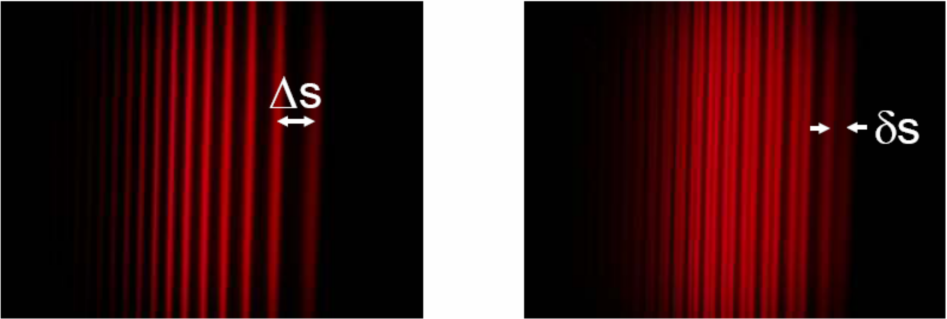
\includegraphics{images/V27_8.pdf}
  \caption{Emissionslinien beim Zeemann-Effekt mit und ohne eingeschaltetem Magnetfeld \cite{anleitung}.}
  \label{abb:streifen}
\end{figure}
